%%% Exemplo de utilização da classe ITA
%%%
%%%   por        Fábio Fagundes Silveira   -  ffs [at] ita [dot] br
%%%              Benedito C. O. Maciel     -  bcmaciel [at] ita [dot] br
%%%              Giovani Volnei Meinertz   -  giovani [at] ita [dot] br
%%%    	         Hudson Alberto Bode       -  bode [at] ita [dot]br
%%%    	         P. I. Braga de Queiroz    -  pi [at] ita [dot] br
%%%    	         Jorge A. B. Gripp         -  gripp [at] ita [dot] br
%%%    	         Juliano Monte-Mor         -  jamontemor [at] yahoo [dot] com [dot] br
%%%    	         Tarcisio A. B. Gripp      -  tarcisio.gripp [at] gmail [dot] com
%%%    	         
%%%
%%%  IMPORTANTE: O texto contido neste exemplo nao significa absolutamente nada.  :-)
%%%              O intuito aqui eh demonstrar os comandos criados na classe e suas
%%%              respectivas utilizacoes.
%%%
%%%  Tese.tex  2016-08-25
%%%  $HeadURL: http://www.apgita.org.br/apgita/teses-e-latex.php $
%%%
%%% ITALUS
%%% Instituto Tecnológico de Aeronáutica --- ITA, Sao Jose dos Campos, Brasil
%%%                   http://groups.yahoo.com/group/italus/
%%% Discussion list: italus {at} yahoogroups.com
%%%
%++++++++++++++++++++++++++++++++++++++++++++++++++++++++++++++++++++++++++++++
% Para alterar o TIPO DE DOCUMENTO, preencher a linha abaixo \documentclass[?]{?}
%   \documentclass[tg]{ita}			= Trabalho de Graduacao
%   \documentclass[tgfem]{ita}	= Para Engenheiras
%   								msc     		= Dissertacao de Mestrado
%   								mscfem   		= Para Mestras
%   								dsc      		= Tese de Doutorado
%   								dscfem   		= Para Doutoras
%   								quali    		= Exame de Qualificacao
%   								qualifem 		= Exame de Qualificacao para Doutoras
% Para 'Draft Version'/'Versao Preliminar' com data no rodape, adicionar 'dv':
%   \documentclass[dsc, dv]{ita} 
% Para trabalhos em Inglês, adicionar 'eng':
%   \documentclass[dsc, eng]{ita}
%		\documentclass[dsc, eng, dv]{ita}
%++++++++++++++++++++++++++++++++++++++++++++++++++++++++++++++++++++++++++++++
\documentclass[tg]{ita}    % ITA.cls based on standard book.cls 
% Quando alterar a classe, por exemplo de [msc] para [msc, eng]) rode mais uma vez o botão BUILD OUTPUT caso haja erro
\usepackage{ae}
\usepackage{graphicx}
\usepackage{epsfig}
\usepackage{amsmath}
\usepackage{amssymb} 
\usepackage{subfig}
\usepackage{multirow}
\usepackage{float}
\usepackage{minted}

%++++++++++++++++++++++++++++++++++++++++++++++++++++++++++++++++++++++++++++++
% Espaçamento padrão de todo o documento
%++++++++++++++++++++++++++++++++++++++++++++++++++++++++++++++++++++++++++++++
\onehalfspacing

%singlespacing Para um espaçamento simples
%onehalfspacing Para um espaçamento de 1,5
%doublespacing Para um espaçamento duplo

%++++++++++++++++++++++++++++++++++++++++++++++++++++++++++++++++++++++++++++++
% Identificacoes (se o trabalho for em inglês, insira os dados em inglês)
% Para entradas abreviadas de Professora (Profa.) em português escreva: Prof$^\textnormal{a}$.
%++++++++++++++++++++++++++++++++++++++++++++++++++++++++++++++++++++++++++++++
\course{Engenharia de Computação} % Programa de PG ou Curso de Graduação

% Autor do trabalho: Nome Sobrenome
\authorgender{masc}                     %sexo: masc ou fem
\author{Miguel Macedo de Araújo}{Neto}
\itaauthoraddress{Rua H8A, 113}{12.228-460}{São José dos Campos--SP}

% Titulo da Tese/Dissertação
\title{Automatização do Conferimento Patrimonial do ICEA usando Smartphones Android}

% Orientador
\advisorgender{masc}                    % masc ou fem
\advisor{Prof.~Dr.}{José Maria Parente de Oliveira}{ITA}

% Coorientador (Caso não haja coorientador, colocar ambas as variáveis \coadvisorgender e \coadvisor comentadas, com um % na frente)
%\coadvisorgender{fem}									% masc ou fem
%\coadvisor{Prof$^\textnormal{a}$.~Dr$^\textnormal{a}$.}{Doralice Serra}{OVNI}

% Pró-reitor da Pós-graduação
%\bossgender{masc}												% masc ou fem
%boss{Prof.~Dr.}{John von Neumann}

%Coordenador do curso no caso de TG
\bosscoursegender{fem}									% masc ou fem
\bosscourse{Prof.~Dr.}{Cecília de Azevedo Castro César}

% Palavras-Chaves informadas pela Biblioteca -> utilizada na CIP
\kwcip{MAVLink}
%\kwcip{}
%\kwcip{}

% membros da banca examinadora

%\examiner{Prof. Dr.}{Alan Turing}{Presidente}{ITA}
%\examiner{Prof. Dr.}{Linus Torwald}{}{UXXX}
%\examiner{Prof. Dr.}{Richard Stallman}{}{UYYY}
%\examiner{Prof. Dr.}{Donald Duck}{}{DYSNEY}
%\examiner{Prof. Dr.}{Mickey Mouse}{}{DISNEY}

% Data da defesa (mês em maiúsculo, se trabalho em inglês, e minúsculo se trabalho em português) 
\date{11}{junho}{2018}

% Número CDU - (somente para TG)
\cdu{621.38}

% Glossario
\makeglossary
\frontmatter

\begin{document}
% Folha de Rosto e Capa para o caso do TG
\maketitle

% Dedicatoria: Nao esqueca essa secao  ... :-)
\begin{itadedication}
A todos aqueles que acreditaram e acreditam em mim
\end{itadedication}

% Agradecimentos
\begin{itathanks}
M

\end{itathanks}

% Epígrafe
\thispagestyle{empty}
\ifhyperref\pdfbookmark[0]{\nameepigraphe}{epigrafe}\fi
\begin{flushright}
\begin{spacing}{1}
\mbox{}\vfill
{\sffamily\itshape
``As our smartphone becomes even smarter,\\
mobile technology should actually take\\
the burden out of our lives.''\\}
--- \textsc{Peggy Johnson}
\end{spacing}
\end{flushright}

% Resumo
%\begin{abstract}
%\noindent
%%Cartas
%%\end{abstract}

% Abstract
\begin{abstract}
\noindent
Micro Air Vehicle Link is an simple open source protocol that has become popular in applications envolving small unmanned aircraft as drones. The protocol is also known for the lack of strong security measures once that is focused on lightweight communication over a bandwith-constrained channel. This paper overviews the main security issues of the protocol presented in the literature as lack of encryption, implementation flaws and vulnerability to network attacks.
The analysis is supported by software-in-the-loop simulations using the Ardupilot project. Besides this work presents the main aspects to understand the MAVLink protocol and the steps necessary to configure the simulation environment in order to reproduce the analysis. 
\end{abstract}

% Lista de figuras
\listoffigures %opcional

% Lista de tabelas
%\listoftables %opcional

% Lista de abreviaturas
\listofabbreviations
\begin{longtable}{ll}
MAVLink & Micro Air Vehicle Link \\
RPA & Remotely Piloted Aircraft \\
RPAS & Remotely Piloted Aerial System \\

\end{longtable}

 %opcional

% Lista de simbolos
% \listofsymbols
% \begin{longtable}{ll}
$a$ & Cachorro\\
$\textbf{a}$ & Vetor de cachorros\\
\end{longtable}

 %opcional

% Sumario
\tableofcontents

\mainmatter
% Os capitulos comecam aqui

\chapter{Introdução}
Esta seção começa com a motivação para o trabalho. Em seguida, tem-se o objetivo do projeto e a organização deste documento.

\section{Motivação}

A gestão do material carga da Força Aérea é feita com o apoio do Sistema
Integrado de Logística de Material e Serviços - SILOMS, mantido pelo Centro de
Computação da Aeronáutica do Rio de Janeiro - CCA RJ. Hoje este sistema atende de
forma eficaz às necessidades das Organizações Militares (OM) quanto à gestão, entretanto
existem algumas restrições:

\begin{itemize}

	\item A conferência do material permanente é realizada de forma
manual por militares da OM. Depois de localizada a etiqueta, a
descrição é conferida com a relação de material setorial disponibilizada pela
seção de registro. Este processo é demorado, cansativo - dependendo da
quantidade de itens - e sujeito a inúmeros erros durante a execução.

	\item A movimentação dos materiais é dada por um processo
administrativo moroso, no qual passar por diversos agentes da OM, gerando
papel e, consequentemente, arquivos.

\end{itemize}

O SILOMS permite a impressão de etiquetas, com ou sem código de barras, e
permite, inclusão, depreciação, transferência para outros setores e/ou outras Unidades e
baixa. No entanto, as conferências são feitas manualmente por não haver equipamento que se
aproveite da existência dos códigos de barra.

\section{Objetivo}
A proposta de trabalho é a criação de um sistema complementar para gerir os materiais, utilizando-se dos dados do SILOMS e de um aplicativo de celular capaz de ler os códigos de barra já existentes, atualmente não utilizados pelo pessoal interno à OM. Ao ler o código de barras com o aplicativo, o usuário insere informações de localização e estado do material carga, e tais dados são enviados a um servidor local do qual se poderia extrair o relatório de maneira mais simples, poupando tempo e mão de obra . Inicialmente aplicado ao ICEA, o sistema poderia futuramente ser expandido para a FAB como um todo, inclusive integrado ao próprio SILOMS.

\section{Organização do trabalho}

\subsection{Decisões de Projeto}
O Capítulo \ref{chproj} descreve as decisões de projeto, mostrando as razões e os requisitos que levaram a tais escolhas.

\subsection{Desenvolvimento}
O Capítulo \ref{chdev} mostra as ferramentas utilizadas e alguns detalhes do desenvolvimento do projeto.

\subsection{Próximos Passos}
O Capítulo \ref{chroadmap} contém as ideias e projeções para a finalização do projeto, além de correções e refatorações no que já foi feito até o presente momento.

\chapter{Decisões de Projeto} \label{chproj}
Micro Air Vehicle Link is a lightweight header-only protocol used in the bidirectional communications between drones and a Control Ground Station (GCS). In general, the GCS sends commands to control the drone and the drone sends its status information in return. It is a binary telemetry protocol designed for resource-constrained systems and bandwidth-constrained links. Nowadays MAVLink is deployed in two major versions: v1.0 and v2.0, which is backwards-compatible. 
%[https://mavlink.io/en/protocol/overview.html]

MAVLink messages have defined formats in order to be consistent between the systems that use the protocol. These formats can be found in an XML file and can be converted to other languages formats, as C/C++ or Python, using a code generator. Writing a new definition in the XML enables to add new messages to the protocol.

\begin{figure}[ht!]
\centering
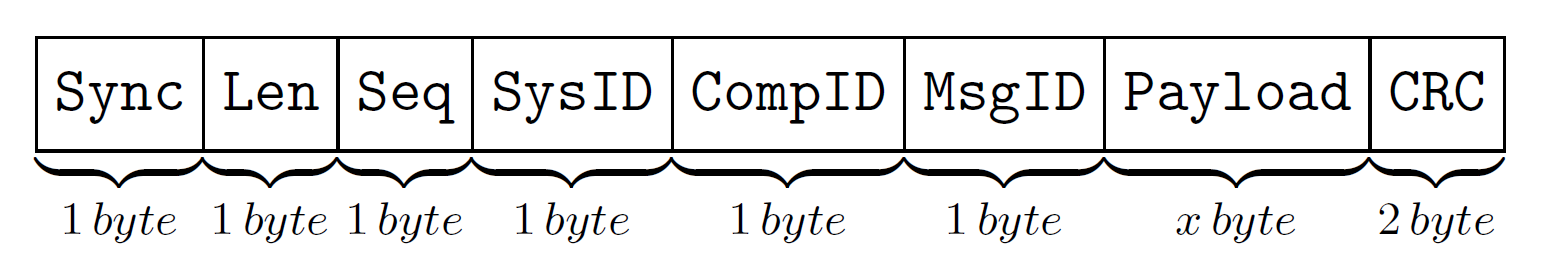
\includegraphics[width=0.75\textwidth]{Cap2/fig_message_structure}
\caption{Structure of a MAVLink v1.0 Message}
\label{fig_message_structure}
\end{figure}

A MAVLink message is a sequence of bytes encoded by a GCS and sent by telemetry over a wireless channel. In this process, the payload is transfomed into a specific data structure and sent in bytes through a channel followed by a checksum for error detection. The data structure of a message can be observed in the figure \ref{fig_message_structure}. The length of a message can vary from 8 to 263 bytes, according to the size of the payload. The fields of a message as shown in \ref{fig_message_structure} are:

\begin{itemize}
\item \textbf{Sync}: is a sequence that indicates the beginning of new MAVLink message. It is also known as protocol magic marker; 
\item \textbf{LEN}: indicates the length of the Payload;
\item \textbf{SEQ}: is the sequence number of the packet. It is used to detect packet loss;
\item \textbf{SysID}: identifies the sending system. It is used to differentiate diferent drones on the same network;
\item \textbf{CompID}: identifies the sending component inside a sending system;
\item \textbf{MsgID}: is the identification of the message, which is used to know how the payload must be interpreted;
\item \textbf{Payload}: data of the message, which contains the parameters. It is no longer than 255 bytes; 
\item \textbf{CRC}: is a 2 bytes checksum used for validation.
\end{itemize}

%The content of this section is based on the documentation provided in the link https://mavlink.io/en/

\section{Differences between versions}

First of all, a MAVLink 2.0 message has more fields than the previous version. The new fields were designed to bring more flexibility and security to the protocol communication.

The new features of MAVLink 2.0 are:
%https://mavlink.io/en/guide/mavlink_2.html
\begin{itemize}
\item More than 256 message IDs (24 bit message ID - over 16 million packets)
	In the version 1.0, only one byte was designed to message IDs  
\item Packet signing (authentication)
\item Extending existing MAVLink messages
\item Variable length arrays (simplified implementation).
\end{itemize}


\section{Working with XML}
MAVLink messages are defined in XML files. The messages that are common to all systems are defined in common.xml and only messages contained in this file are considered standard messages. 
%https://mavlink.io/en/messages/

\section{Adding a new message}

%http://ardupilot.org/dev/docs/code-overview-adding-a-new-mavlink-message.html

Adding a new message to the protocol can be done by following the steps. We will add a new message called NAMEOFMESSAGE to exemplify the tutorial.

\textbf{Step 1:} Install MAVProxy and the lastest version of ArduPilot code.

In section \ref{downloading_the_code} you can find how to clone the code from GitHub. Also check Mavproxy, which can be updated by running the next command line in a Terminal.

\begin{verbatim}
sudo pip install --upgrade mavproxy
\end{verbatim}

\textbf{Step 2:} Decide what type of message you want to add and how it will fit in with the existing MAVLink messages.

\textbf{Step 3:} Add the new message definition to the common.xml or ardupilotmega.xml file in the mavlink submodule;

%\textbf{Step 4:}

\textbf{Step 4:} Add functions to the main vehicle code to handle sending or receiving the command to/from the ground station. 


%%\begin{table}
%%\caption{Exemplo de uma Tabela}
%%\label{minhatab}
%\center
%\begin{tabular}{cccc}
 %  after \\: \hline or \cline{col1-col2} \cline{col3-col4} ...
 %\hline
%	Parametro & Unidade & Valor da simulação & Valor experimental   \\
%	\hline
 % Comprimento, $\alpha$ & $m$ &  $8,23$  & $8,54$ \\
  %Altura, $\beta$ & $m$     &  $29,1$ & $28,3$\\
	%Velocidade, $v$ & $m/s$  &  $60,2$ & $67,3$\\
	%\hline
%\end{tabular}
%\end{table}







\chapter{Desenvolvimento} \label{chdev}
This chapter explains how to set up SITL ArduPilot Simulator in a virtual machine environment on Windows following the instructions the Ardupilot Dev Team tutorial. The tutorial was tested on Windows 10 with Oracle VM VirtualBox 5.2.12 and Ubuntu 16.04.
%http://ardupilot.org/dev/docs/setting-up-sitl-on-linux.html

Software In The Loop simulator allows to run ArduPilot code without any hardware. So SITL simulation is ideal to test new featues and changes in the code during development.

\section{Downloading the ArduPilot Code} \label{downloading_the_code}
%http://ardupilot.org/dev/docs/setting-up-sitl-on-linux.html
The ArduPilot project uses git for source code management and GitHub for source code hosting. To install git use the commands in the terminal:  %http://ardupilot.org/dev/docs/where-to-get-the-code.html#where-to-get-the-code

\begin{verbatim}
sudo apt-get update
sudo apt-get install git
\end{verbatim}

Now you have to get a copy of the ardupilot git repository. Open the terminal and run:
\begin{verbatim}
git clone git://github.com/ArduPilot/ardupilot.git
cd ardupilot
git submodule update --init --recursive
\end{verbatim}

Install required packages using the script \textit{install-prereqs-ubuntu.sh}  located in \textit{ardupilot/Tools/scripts}. Go to the directory you cloned ardupilot into and use the following command line. It can take a while depending on your internet connexion. Don't forget to accept the changes when asked.
\begin{verbatim}
cd ardupilot/Tools/scripts/install-prereqs-ubuntu.sh
\end{verbatim}

Now you have to add the following lines to the end of your \textit{.bashrc} file in your home directory. Notice the . on the start of that filename. Also, this is a hidden file, so if you’re using a file manager, make sure to turn on “show hidden files”.

\begin{verbatim} 
export PATH=$PATH:$HOME/ardupilot/Tools/autotest
export PATH=/usr/lib/ccache:$PATH
\end{verbatim}

Save the \textit{.bashrc} file and open the terminal. Then reload your PATH by using the “dot” command in a terminal:

\begin{verbatim} 
. ~/.bashrc
\end{verbatim}
If you don't change the  \textit{.bashrc} file you will not be able to use \textit{sim\_vehicle.py} as described in the next section.

\section{How to start SITL simulator}
In the terminal, go to the directory of the vehicle you want to make a simulation with. For example, for the multicopter code use the command line:
\begin{verbatim}
cd ardupilot/ArduCopter
\end{verbatim}

Then start the simulator using \textit{sim\_vehicle.py}. The first time you run it you should use the -w option to wipe the virtual EEPROM and load the right default parameters for your vehicle.
\begin{verbatim}
sim_vehicle.py -w
\end{verbatim}

After the default parameters are loaded you can start the simulator normally. First kill the sim\_vehicle.py you are running using Ctrl-C. Then:
\begin{verbatim}
sim_vehicle.py --console --map
\end{verbatim}

\section{FlightGear 3D View}  \label{sec_flightgear_view}

It is possible to install FlightGear Flight Simulator to display a 3D simulation of the vehicle and its surroundings. To install FlightGear from terminal use next command line. It may take a few minutes to finish the download.

\begin{verbatim}
sudo apt-get install flightgear
\end{verbatim}

If you want to run the simulation including the FlightGear 3D view, you need to open a new terminal, go to the directory \textit{/ardupilot/Tools/autotest/} and open \textit{fg\_quad\_view.sh} (Copter). This will start FlightGear. The next steps show the procedure to run the simulation.

\begin{enumerate}
\item In a terminal use the command lines:
\begin{verbatim} 
cd ardupilot/Tools/autotest
./fg_quad_view.sh 
\end{verbatim}

\item In other terminal:
\begin{verbatim} 
cd ardupilot/Ardu
sim_vehicle.py -j4 -L KSFO --map --console
\end{verbatim}

\end{enumerate}

In the step 2, KSFO indicates the location where the simulation will take place. FlightGear will always start by loading scenery at KSFO (San Francisco International Airport) but will change to the selected scenery once SITL is started.
If the vehicle appear to be hovering in space (no scenery) then you don't have the files for that location, but you can download it after. 

\subsection{Adding a new location to FlightGear}
	
    New locations are hard-coded into a file. This section shows how to add a new location. We will call the location as KSFO\_PAPI, because it will be next to PAPI lights in a lane of KSFO.
    
    In the directory \textit{ardupilot/Tools/autotest} find the \textit{locations.txt} file. This file contains all the locations you can choose for simulation. Each line follows the sintaxe:

\begin{verbatim}
#NAME=latitude,longitude,absolute-altitude,heading
\end{verbatim}  

Then add to the file the next line. 
\begin{verbatim}
KSFO_PAPI = 37.6136, -122.357, 5.3, 297.9
\end{verbatim}  
When you run the simulation in KSFO\_PAPI location using the steps shown in section \ref{sec_flightgear_view}, FlightGear environment will be as in figure \ref{fig_papi_lights}.

\begin{figure}[ht!] 
\centering
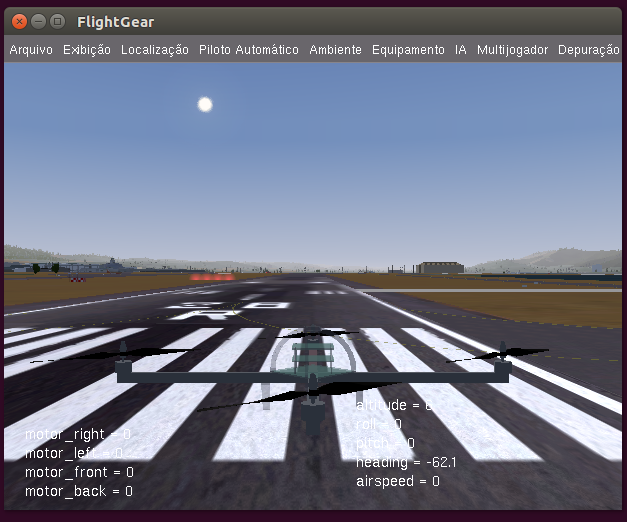
\includegraphics[width=1.0\textwidth]{Cap3/fig_papi_lights}
\caption{Image from FlightGear simulator running in SITL. Observe four red lights (PAPI) in the left of the lane. }
\label{fig_papi_lights}
\end{figure}






\chapter{Próximos Passos} \label{chroadmap}
%\section{Conclusão}
After setting up the simulation environment and studying about MAVLink, the next steps is to check in the literature the main complains about MAVLink security in order to start to develop a more structured analysis. The analysis aims to exploit MAVLink vulnerabilities inside simulations in order to sustain conclusions.

During this process is expected to expand the MAVLink documentation this work want to present, including examples of normal use of the protocol in simulated environment. All the necessary steps to reproduce the simulations in other computers will be presented in order to help in related projects.


% REFERENCIAS BIBLIOGRAFICAS
\renewcommand\bibname{\itareferencesnamebabel} %renomear título do capítulo referências
\bibliographystyle{abnt-alf}
\bibliography{Referencias/referencias}

% Apendices
%\appendix
%\chapter{Topicos de Dilema Linear} %opcional
%\section{Uma Primeira Seção para o Apêndice}

A matriz de Dilema Linear $M$ e o vetor de torques inerciais $b$,
utilizados na simulação são calculados segundo a formulação 
abaixo:
\begin{equation}
M=\left[ \begin{array}{ccc}
M_{11} & M_{12} & M_{13} \\
M_{21} & M_{22} & M_{23} \\
M_{31} & M_{32} & M_{33}
\end{array} \right]
\end{equation}

\begin{figure}[h]
\centering
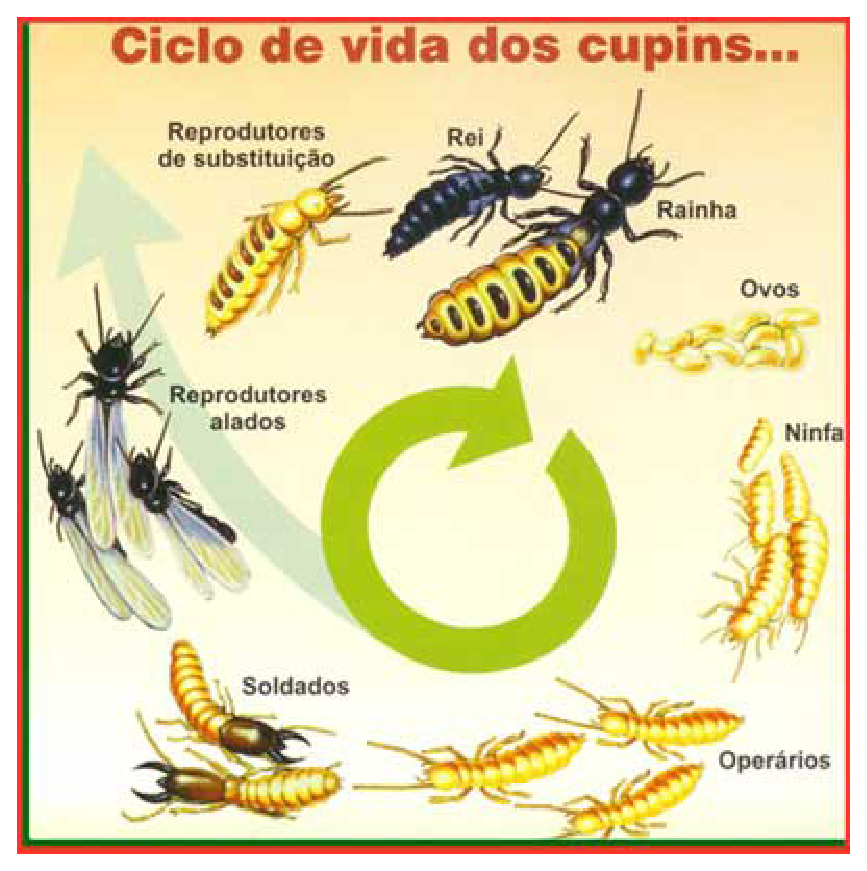
\includegraphics[height=5cm, width=5cm]{ApeA/pragas_ciclo_cupim}
\caption{Uma figura que está no apêndice}\label{FD}
\end{figure}


% Anexos
%\annex
%\chapter{Exemplo de um Primeiro Anexo} %opcional
%% Texto do Primeiro Anexo
\section{Uma Seção do Primeiro Anexo}
% Texto da primeira secao do primeiro anexo
Algum texto na primeira seção do primeiro anexo.



% Glossario
%\itaglossary
%\printglossary

% Folha de Registro do Documento
% Valores dos campos do formulario
% \FRDitadata{ de Novembro de 2018}
% \FRDitadocnro{DCTA/ITA/DM-018/2015} %(o número de registro você solicita a biblioteca)
% \FRDitaorgaointerno{Instituto Tecnológico de Aeronáutica -- ITA}
%Exemplo no caso de pós-graduação: Instituto Tecnol{\'o}gico de Aeron{\'a}utica -- ITA
% \FRDitapalavrasautor{MAVLink; Drones; Software-In-The-Loop}
% \FRDitapalavrasresult{Cupim; Dilema; Construção}
%Exemplo no caso de graduação (TG):
% \FRDitapalavraapresentacao{Trabalho de Graduação, ITA, São José dos Campos, 2018. \NumPenultimaPagina\ páginas.}
%Exemplo no caso de pós-graduação (msc, dsc):
%\FRDitapalavraapresentacao{ITA, São José dos Campos. Curso de Engenharia da Computação. Área de Sistemas Aeroespaciais e Mecatrônica. Orientador: Prof.~Dr. Juliana de Melo Bezerra. Defesa em 29/11/2018. Publicada em 25/03/2015.}
% \FRDitaresumo{Cartas}
%  Primeiro Parametro: Nacional ou Internacional -- N/I
%  Segundo parametro: Ostensivo, Reservado, Confidencial ou Secreto -- O/R/C/S
% \FRDitaOpcoes{N}{O}
% Cria o formulario
% \itaFRD

\end{document}
% Fim do Documento. O massacre acabou!!! :-)
